\chapter{User's manual}
This chapter describes how to use Origamist Viewer and Origamist Editor.

Origamist applications are designed to help with creating and distribution of origami model manuals. You can find a lot of such manuals on the web or in books, but none of them is 3D! Origamist provides a full 3D preview of every step in the manual, and has excellent export options. So, from the 3D manual, you can export the standard manual formats, such as PDF manuals or images, but you can also generate some fancy formats (SVG - it is vector graphics format), or you can even generate the whole process as an animation! Cool! Origami Editor provides support for creation of the 3D manual, so you can play with paper on your screen as if you held it in your hands!

Also, everyone can assemble his own sets of origami models (called listings here), sorted into categories, and distribute them wherever he wants.

\section*{Installation \& supported platforms}
How to install Origamist applications? Well, no installation is needed! Everything you need is a web browser with Java installed (ensure you have at least Java 6 or 1.6). Origamist Viewer and Editor are designed as web applets, so they can be loaded directly into a webpage. As Origamist is Java application, it is multiplatform - runs on Windows, Mac, Linux\footnote{Linux users, please use the Oracle JRE version of Java, other versions, such as Icedtea Java have problems with Origamist}, Solaris and maybe further platforms.

The only thing you have to do, that isn't automatised, is pressing Yes or Run in a security dialog which appears shortly after the applet starts loading.

There are another ways of launching Origamist. It is also available as a JNLP application, which means it can be installed on your computer and the be run as a standalone application without the need to launch web browser. If you want to use it this way, just click a link to the Origamist JNLP file you can find on the web, and the installation will start.

As the last option you can download Origamist and all of its libraries, and run it as a standard Java application (it is packed in a JAR file, so it should be sufficient to type the `java -jar OrigamistViewer.jar' command and that should be everything).

\section{Viewer}
It will be best to describe the viewer's controls on screenshots, because there is no complex functionality. So, look over figures \ref{fig:viewer} to \ref{fig:settings}.

\begin{figure}
	\centering
	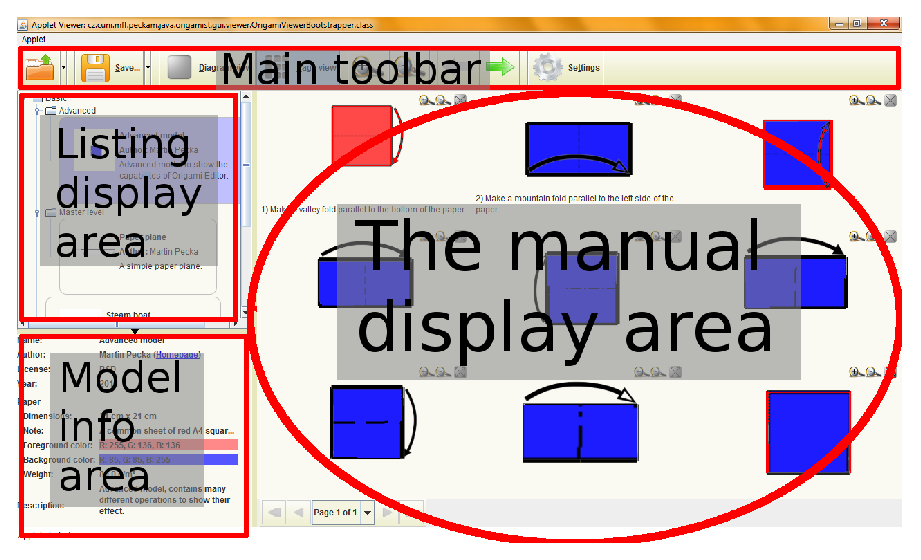
\includegraphics[width=150mm]{images/viewer-overall}
	\label{fig:viewer}
	\caption{The viewer's main window. You see the main areas of the application.}
\end{figure}

\begin{figure}
	\centering
	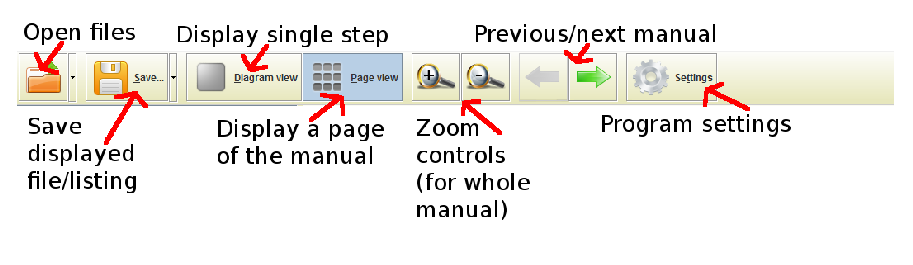
\includegraphics[width=150mm]{images/viewer-toolbar}
	\label{fig:viewerToolbar}
	\caption{Viewer's toolbar. Most buttons are either intuitive or described later. Diagram View and Page View buttons switch the view modes - diagram mode displays only one step at a time in the Manual display area, whereas page mode displays a whole page of the manual in that area. The zoom buttons in this toolbar set zoom for all steps from the current diagram, so they are an easy way how to zoom all steps at once.}
\end{figure}

\begin{figure}
	\centering
	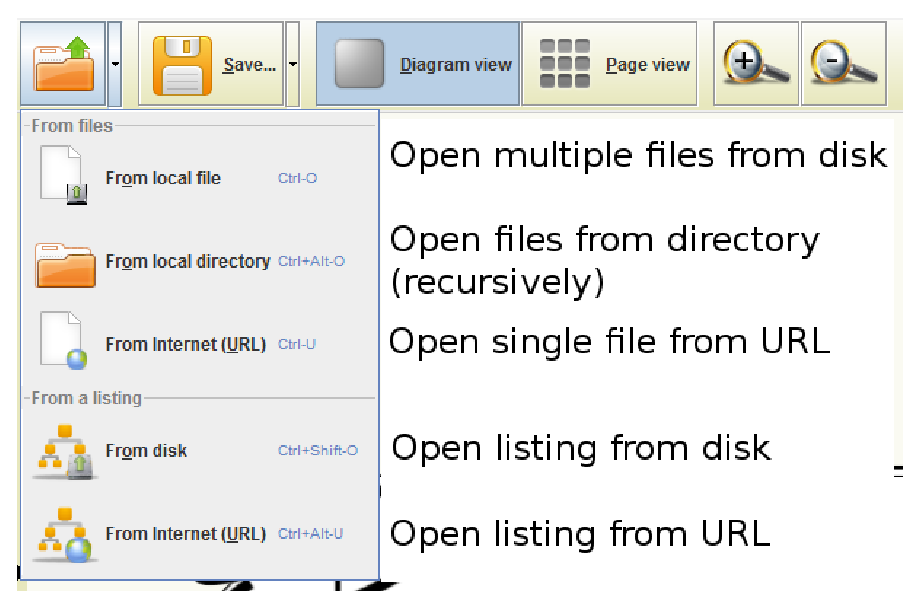
\includegraphics[width=80mm]{images/viewer-open}
	\label{fig:viewerOpen}
	\caption{Open file dialog. First three buttons are for opening models (multiple local models by the first option, a whole directory of models by the second one, and a single model from Internet by the third one). Last two buttons are intended to handle loading of whole listings. So you can either load a listing from the local computer, or from Internet.}
\end{figure}

\begin{figure}
	\centering
	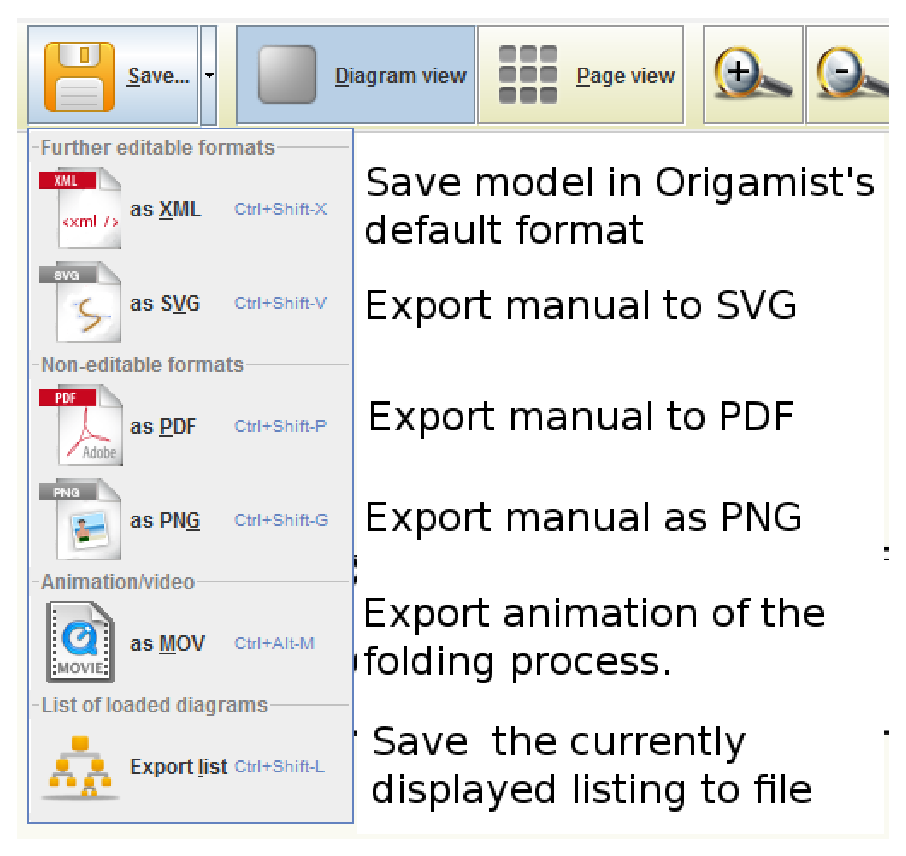
\includegraphics[width=80mm]{images/viewer-save}
	\label{fig:viewerSave}
	\caption{The save options of viewer. In the top-bottom order, they are: Save as XML, which is Origamist's default format and allows the model to be again loaded in Origamist applications; Save as SVG, which save the manual as several SVG files (one per manual page; the filename entered to the save dialog will be used as a pattern for filenames of the generated files); Save as PDF, which saves the manual to a single PDF file; Save as PNG, which saves the manual to a series of PNG images (one per manual page; again, the entered filename serves as pattern); Sase as MOV, which generates an animation of the folding process into a Quicktime MOV video file; Export the currently loaded listing (can be used to either save a remotely loaded listing, or to generate a listing from the loaded directory structure). After you select to export the model to a format, export options dialog will appear allowing you to specify the details of the exported manual (such as the used steps' descriptions language).}
\end{figure}

\begin{figure}
	\centering
	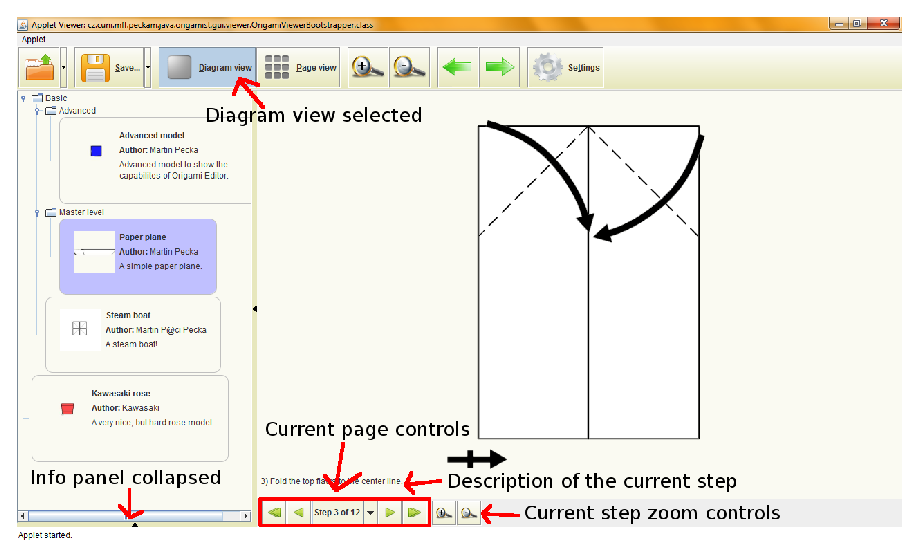
\includegraphics[width=150mm]{images/viewer-diagram-mode}
	\label{fig:viewerDiagram}
	\caption{The viewer in diagram mode, where only one step is displayed at once. You may notice the info panel is collapsed by clicking the small arrow on the top of it. You also see the step controls which allow to browse the manual, description of the currently displayed step, and the zoom controls for just this one step (the zoom isn't applied globally).}
\end{figure}

\begin{figure}
	\centering
	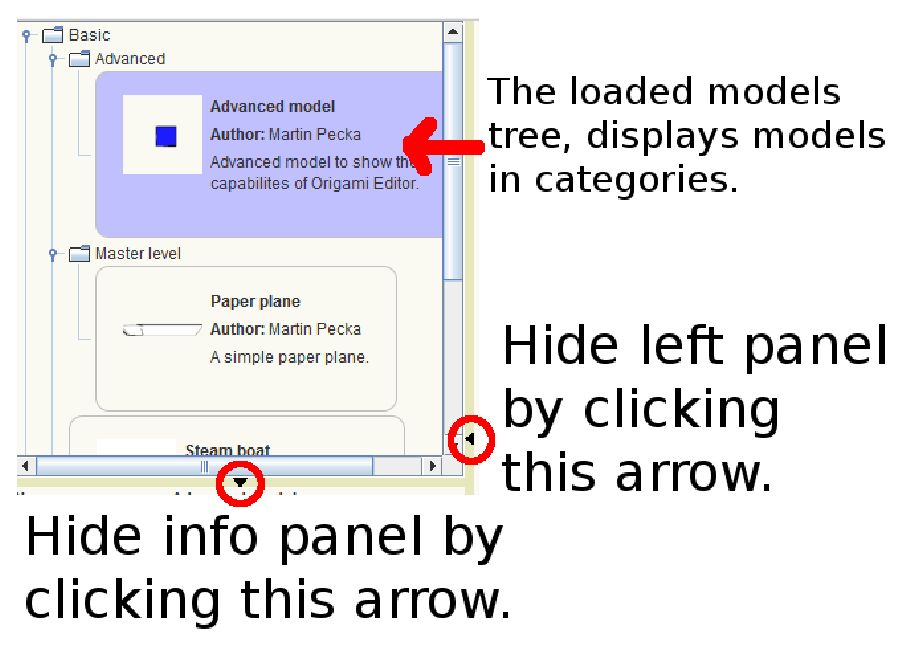
\includegraphics[width=100mm]{images/viewer-models-tree}
	\label{fig:viewerTree}
	\caption{The loaded models tree displays all loaded models (either from a listing or from directories). If the models are loaded from directories, than the directory names will be displayed as category names, otherwise the category names will be loaded from the listing. You can hide the loaded models tree (along with model info panel) by clicking the small arrow on its right side.}
\end{figure}

\begin{figure}
	\centering
	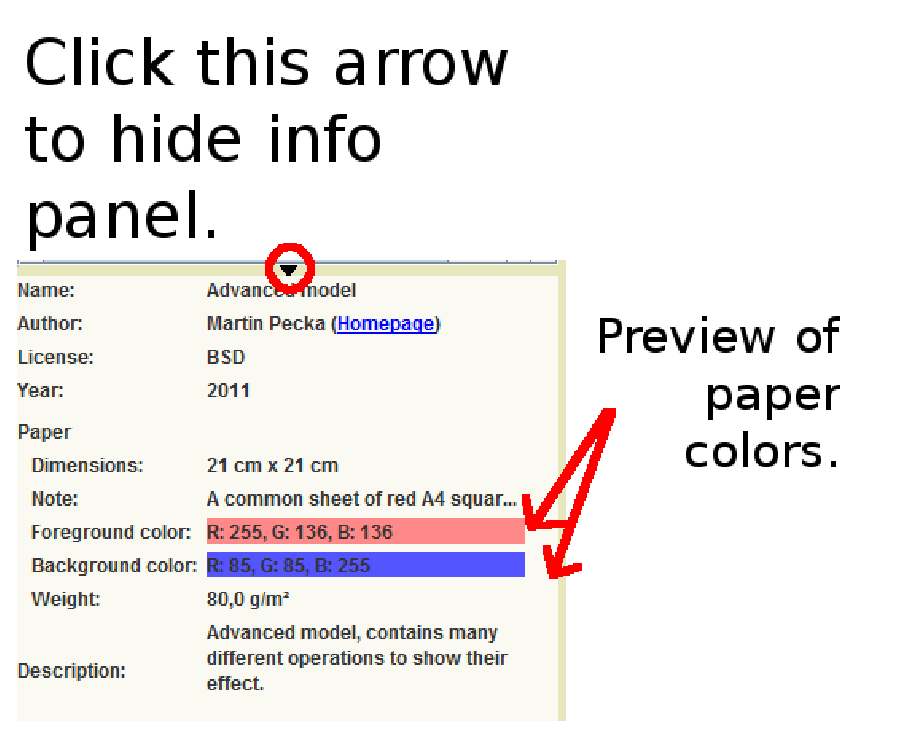
\includegraphics[width=100mm]{images/viewer-model-info}
	\label{fig:viewerInfo}
	\caption{The model info panel. Displays some basic information about the currently displayed model. Notice the preview of paper foreground/background colors, by which the author says how the used paper should be colored. You may show/hide this panel by clicking the small arrow on its top.}
\end{figure}

\begin{figure}
	\centering
	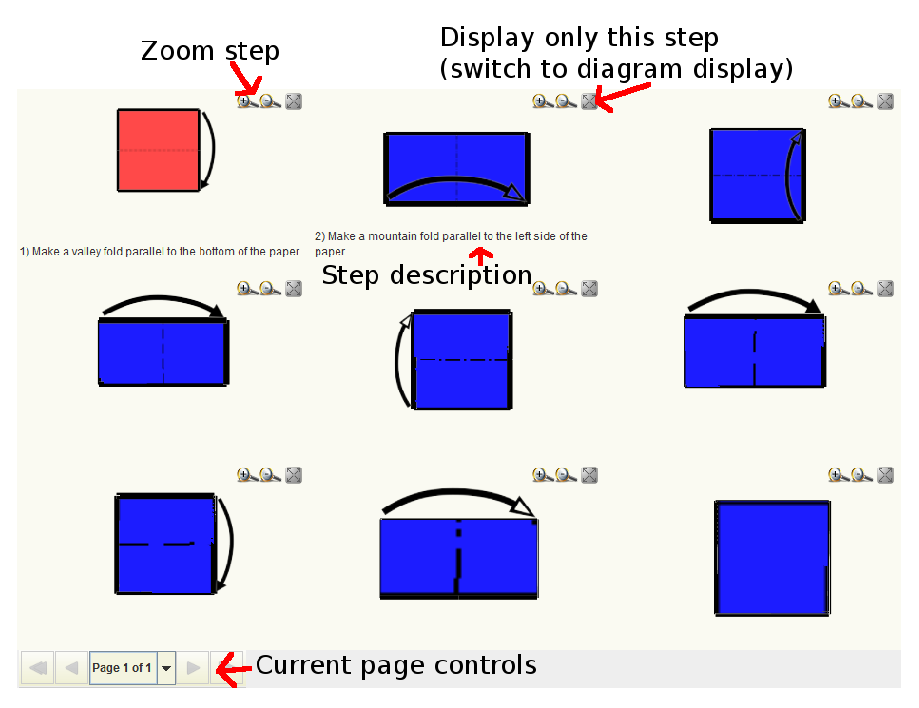
\includegraphics[width=150mm]{images/viewer-model-page}
	\label{fig:viewerModel}
	\caption{Manual display area in page mode, which shows a single page from the manual (the definition of the page layout, number of steps per page and so on is saved in the loaded model). Every step has its small toolbar with zoom buttons (these buttons zoom only that one particular step), and the fullscreen button, which displays the particular step in diagram mode.}
\end{figure}
\begin{figure}
	\centering
	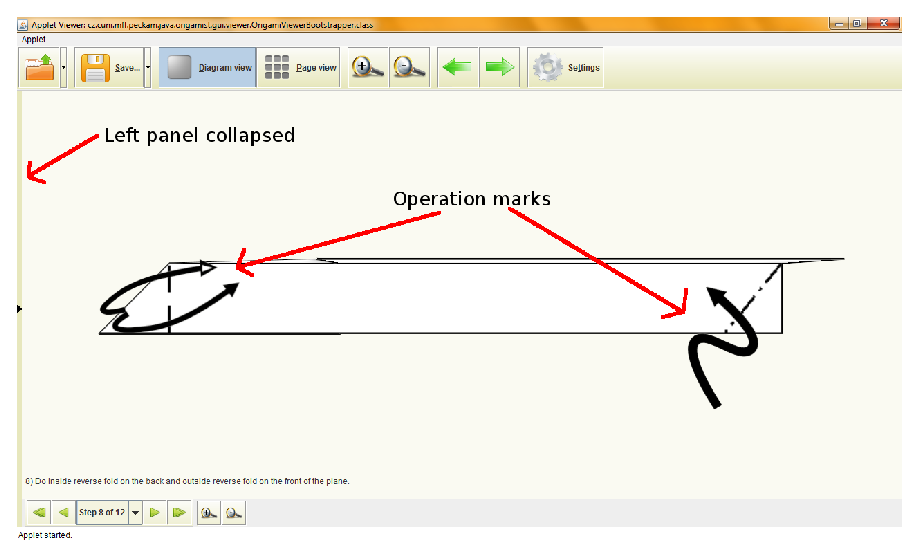
\includegraphics[width=150mm]{images/viewer-left-collapsed}
	\label{fig:viewerCollapsed}
	\caption{The viewer with the left panel completely collapsed (you can either do it manually, or it is done automatically if you load only a single model). Notice the operation marks designing what operations are done in this step.}
\end{figure}

\begin{figure}
	\centering
	
\includegraphics[width=100mm]{images/settings}
	\label{fig:settings}
	\caption{Settings of the application. Program language is the language of program controls and dialogs (only several languages are available, and if the yours is not, English is selected), whereas language of diagrams is the preferred language of the steps' descriptions.}
\end{figure}


\section{Editor}
Origamist editor is for creating new and editing existing origami models. It also has the same export options as viewer (except listing export, since the editor doesn't handle listings).

\begin{figure}
	\centering
	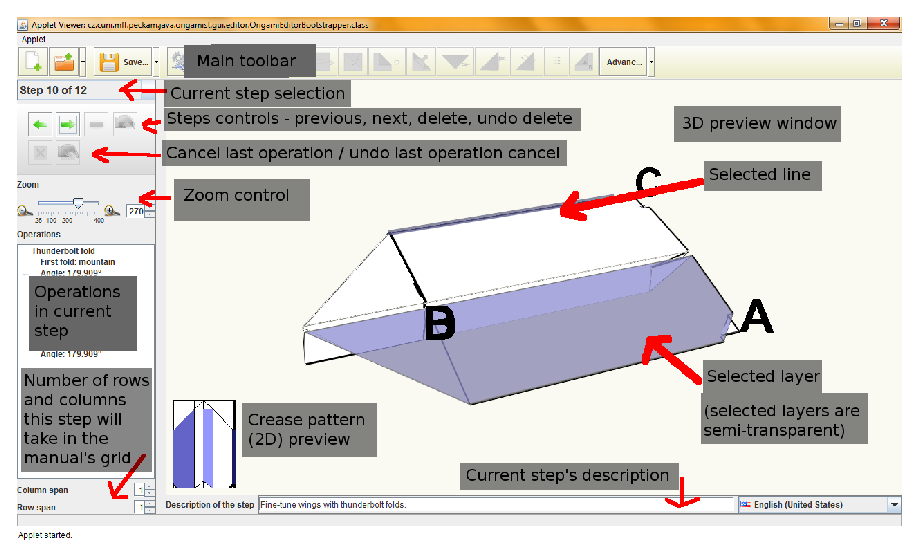
\includegraphics[width=150mm]{images/editor-preview}
	\label{fig:editorPreview}
	\caption{Different layers that can be bent}
\end{figure}

To create a new model, click the New button (the leftmost in toolbar), and a dialog asking for inputting several information will open. Detailed description of this dialog is included in the PDF with Origamist manual you should be able to get from the same source you have got Origamist from; although the dialog contains many fields and may look complex, it just asks the basic information - your name, name of the model, some description of the model, type of the paper the model is created from and so on. Most of the fields are optional, so it is fine to leave them blank. Please, pay attention to the License fields. Origamist wants that every model has clear rules of its usage. You can choose among several licenses. If you have invented the model, you can even issue it under the Public domain, which means that no restrictions apply to the model. If you just crate a model you have learnt from someone or from another manual, you should consider asking the original author if you can distribute the manual, and under which terms (if you just create the model for your own fun, you don't have to bother selecting a license, but then you cannot distribute it).

Now you can take a look at figures \ref{fig:editorPreview} to \ref{fig:editorLines} to get used with the editor environment.

\begin{figure}
	\centering
	
\includegraphics[width=150mm]{images/editor-toolbar}
	\label{fig:editorToolbar}
	\caption{Different layers that can be bent}
\end{figure}

\begin{figure}
	\centering
	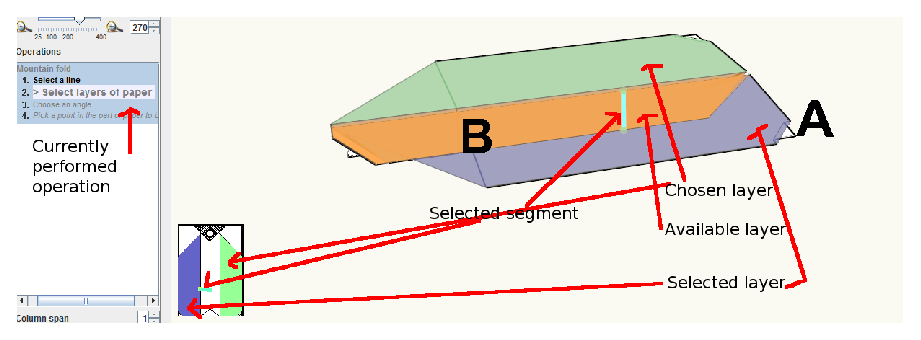
\includegraphics[width=150mm]{images/editor-layers}
	\label{fig:editorLayers}
	\caption{Different layers that can be bent}
\end{figure}

\begin{figure}
	\centering
	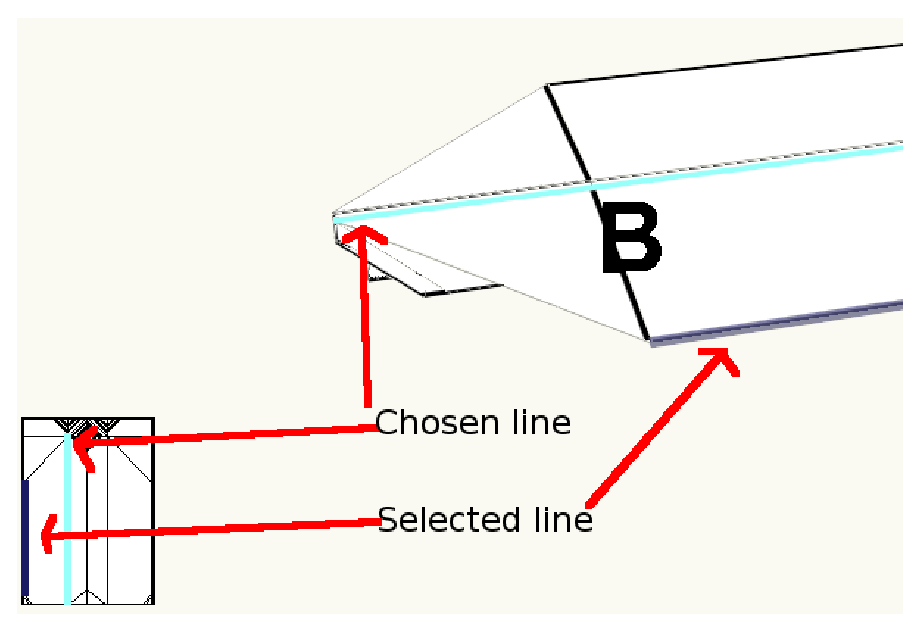
\includegraphics[width=100mm]{images/editor-lines}
	\label{fig:editorLines}
	\caption{Different layers that can be bent}
\end{figure}

\subsection{Creating the model}
After you have created a new or opened an existing model, you can edit it. More precisely - you can edit only its last step, so if you have loaded an existing model, all the operation buttons will be disabled until you select the last step.

You can select any operation among the operation buttons in the toolbar, and apply that operation to the model. If you don't know what that operation means, you can try reading the tooltip of the button (which shows when you hover it with mouse), and if even that doesn't help, then please refer to an origami book or a webpage dedicated to origami (Origamist uses a standard origami nomenclature, though, there isn't only one standard nomenclature in origami).

After selecting an operation, an item appears in the left operations list, that tells you what the editor needs to know to perform the operation. These are basically 1 to 5 steps where you select lines, points, paper layers, angles and so on.

Take a look in the upper right corner of editor, you can see a small help there. In this area, tips related to the currently performing operation appear. So, if you do eg. a mountain fold, the first tip in this area will tell you that it is needed to select a line, along which the fold will be bent; the second one will tell you to select the layers of paper the operation should affect, and so on.

Let's call these steps needed to be done to perform an operation as the operation arguments. If you finish filling up one operation argument, you can move to the next argument by pressing Space or Enter. If you have just completed the last argument, the operation will be performed after pressing Space or Enter. If you have done a mistake, you can press Esc to return to the previous argument (if you are on the first argument, the whole operation will be cancelled).

\subsection{How to select points, lines etc.?}
So, if an operation argument requires to select some lines, points or layers of paper, what are you supposed to do? 

First (without an operation selected) notice, that pressing the middle mouse button changes the mouse cursor. The standard cursor selects points, the next is the crosshair cursor, which selects lines, and the last one is the hand cursor, which selects layers of paper.

So, if you are asked to select something, you must switch to the right selection mode (however, most operation arguments will do the switch automatically).

Then you can begin selecting. You select/deselect by left-clicking. If there are multiple items under the cursor (eg. four layers of paper), use mouse wheel to choose among them (exactly one of the items will be highlighted, and that is the one that will be selected when you click). You can perform the selection both in the 3D preview or in the 2D preview (combining these two you should be able to select precisely those items you want to). Sorry, but there is no support for keyboard selection (but you can emulate it using keyboard-mouse emulation your operating system surely provides).

Now, some terminology is needed to be declared. Items can be either non-selected, selected, available or chosen (I know that there's little difference between selected and chosen, but, please, treat it like terminology). Non-selected items have their default color and are opaque. Selected items are dark blue and semi-transparent (points are dark green). Only layers can be available, and available layers are orange and semi-transparent. Chosen items are green or azure, and chosen layers are semi-transparent. Every item can be highlighted (be the active one under the cursor), such items are opaque and are `lifted up' in the foreground.

One more term needs to be defined - a layer of paper. You can imagine it as a straight (unfolded) part of paper. So, if you eg. fold the paper in half and again in half, you get 4 layers of paper.

What does this terminology mean? If you want to fill up an operation's argument, you need to choose the desired item. If no operation is being filled-up right now, you always only select the items. You also select items if you are in other selection mode than the current argument requires (eg. if you have to choose a point, and switch to line selection, you no longer choose - you select). Available layers will be defined later.

\subsubsection{How to choose points}
Points can only be chosen in point selection mode. However, both line and layer selection modes are also available. You can select lines or layers to constrain the places where a point can be selected. So, if it is hard to select the correct point you want, but it easy to select the layer it lies in, first select the layer and then only points lying in this layer can be chosen. You can do the same using lines.

Note that you can only select points on edges and creases, you cannot select points lying `inside' a layer.

When you choose points, some of them are magnetic to help you. Magnetic points are squares (instead of circles). The snap to the start- and end-points of lines, and also to the exact halves of lines. Also, magnetic points will be shown to allow you select 90� angles.

\subsubsection{Hot to choose lines?}There are two types of lines - those existing, and those that don't exist. You can always choose a line in the line selection mode, and you can constrain it by selecting a layer (if a layer is selected, only lines going through this layer can be chosen).

There is one more option how to select a line (a non-existing one). You can switch to the point selection mode and select two border points of the line. Here available layers come to the scene. After you select the first point, some layers will be made available. Then, only points lying in the available layers can be chosen as the opposite end of the line.

\subsubsection{How to choose layers?}
There's no magic behind layers selection. Just highlight the layer you want to choose, and click on it. Use mouse wheel to iterate over all layers under the mouse cursor.

What is needed to be known of layer selection, is what is it for. Well, imagine you have the paper twice folded in halves. It has four layers. Now you want to fold it again in half. Now you have two options - you can either fold the top two layers, the bottom two layers, or all four layers. That is what are layers for. If you select layers affected by an operation, you always select only those layers that are crossed by the fold line. The rest of affected layers (those who are firmly attached to the already affected layers) are detected automatically.

Be careful when thinking about what layers to select, because badly selected layers won't allow the operation to be completed.

\section{How to compose it together?}
Now you can fill up every argument an operation may need. So you are ready to create origami models! Every operation shows a description of the meaning of the current argument (in the top right corner), so you shouldn't have problems with understanding what is the current argument needed for.

\section{Use the New step button and fill up step descriptions}
It is a good practice not to do many operations in one step. If they are repeating operations, you can hide them under the repeat operation. So, if you have done a small number of operations, fill in the step's textual description (in the bottom) and click the Next step button (which changes to Add new step button in the last step). That's all. And --- don't forget to save the final work!

\section{A little tutorial}
The following figures show a step-by-step tutorial of how to fold a frog base.
Enjoy and good luck!

\begin{figure}
	\centering
	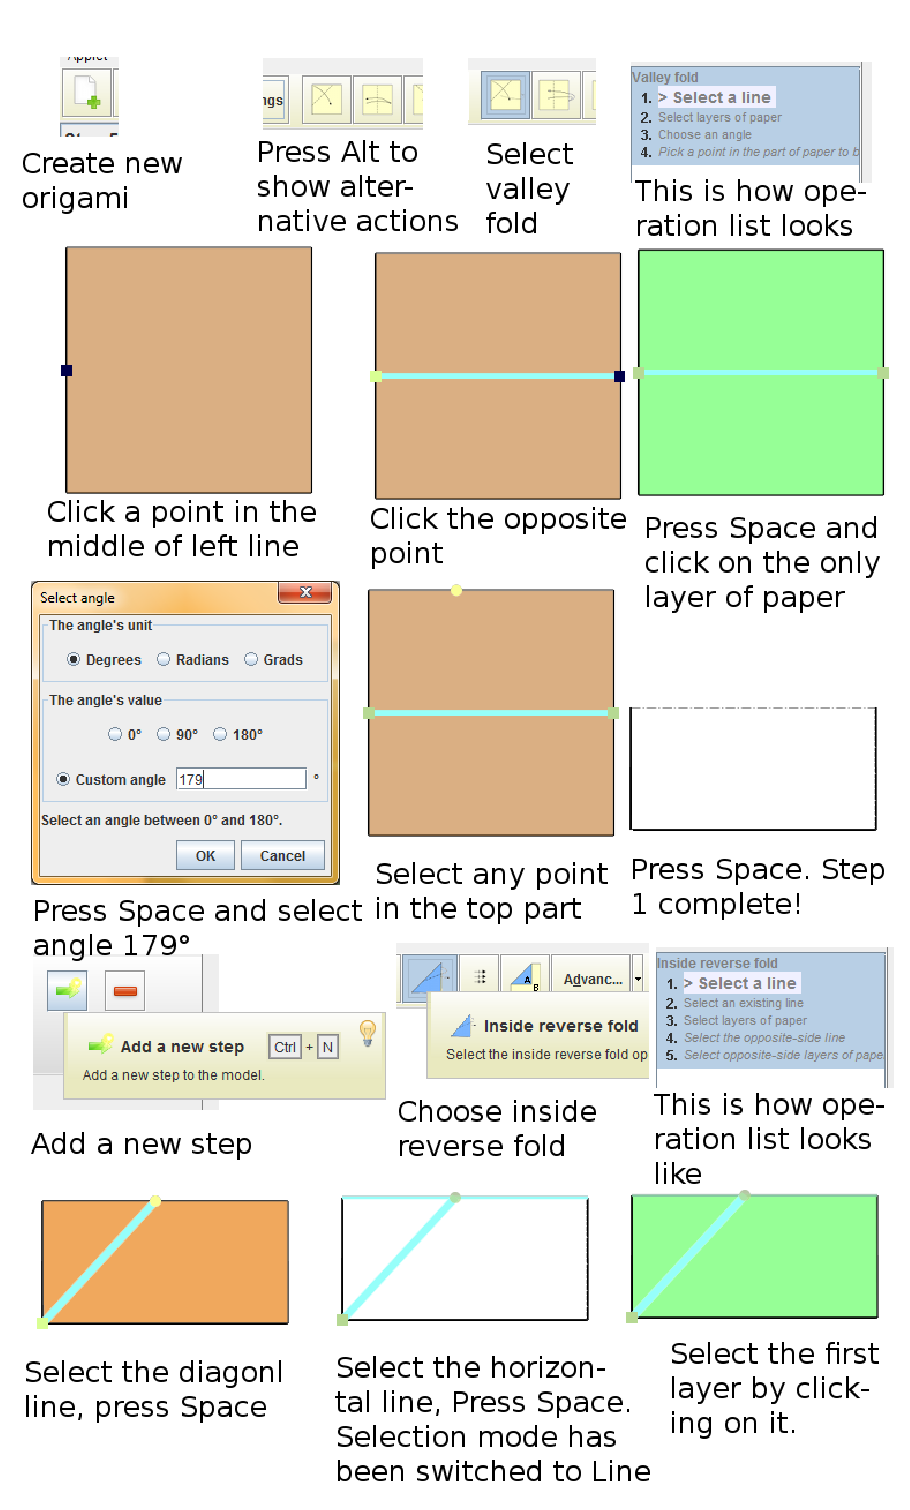
\includegraphics[width=140mm]{images/frog-tutorial}
	\label{fig:tutorial1}
	\caption{Frog base tutorial, part 1}
\end{figure}

\begin{figure}
	\centering
	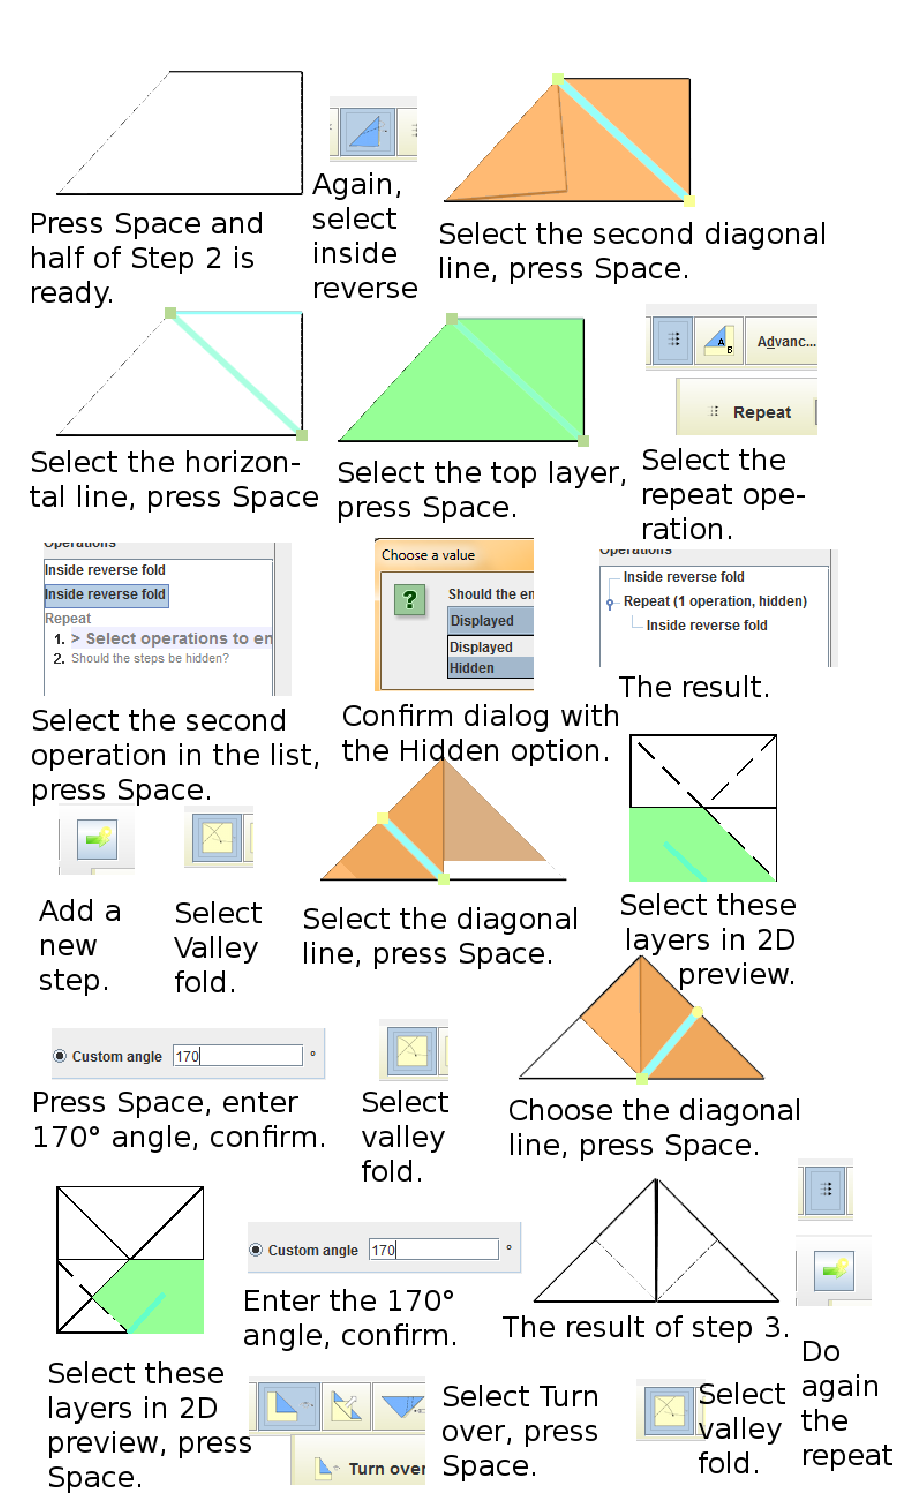
\includegraphics[width=140mm]{images/frog-tutorial2}
	\label{fig:tutorial2}
	\caption{Frog base tutorial, part 2}
\end{figure}

\begin{figure}
	\centering
	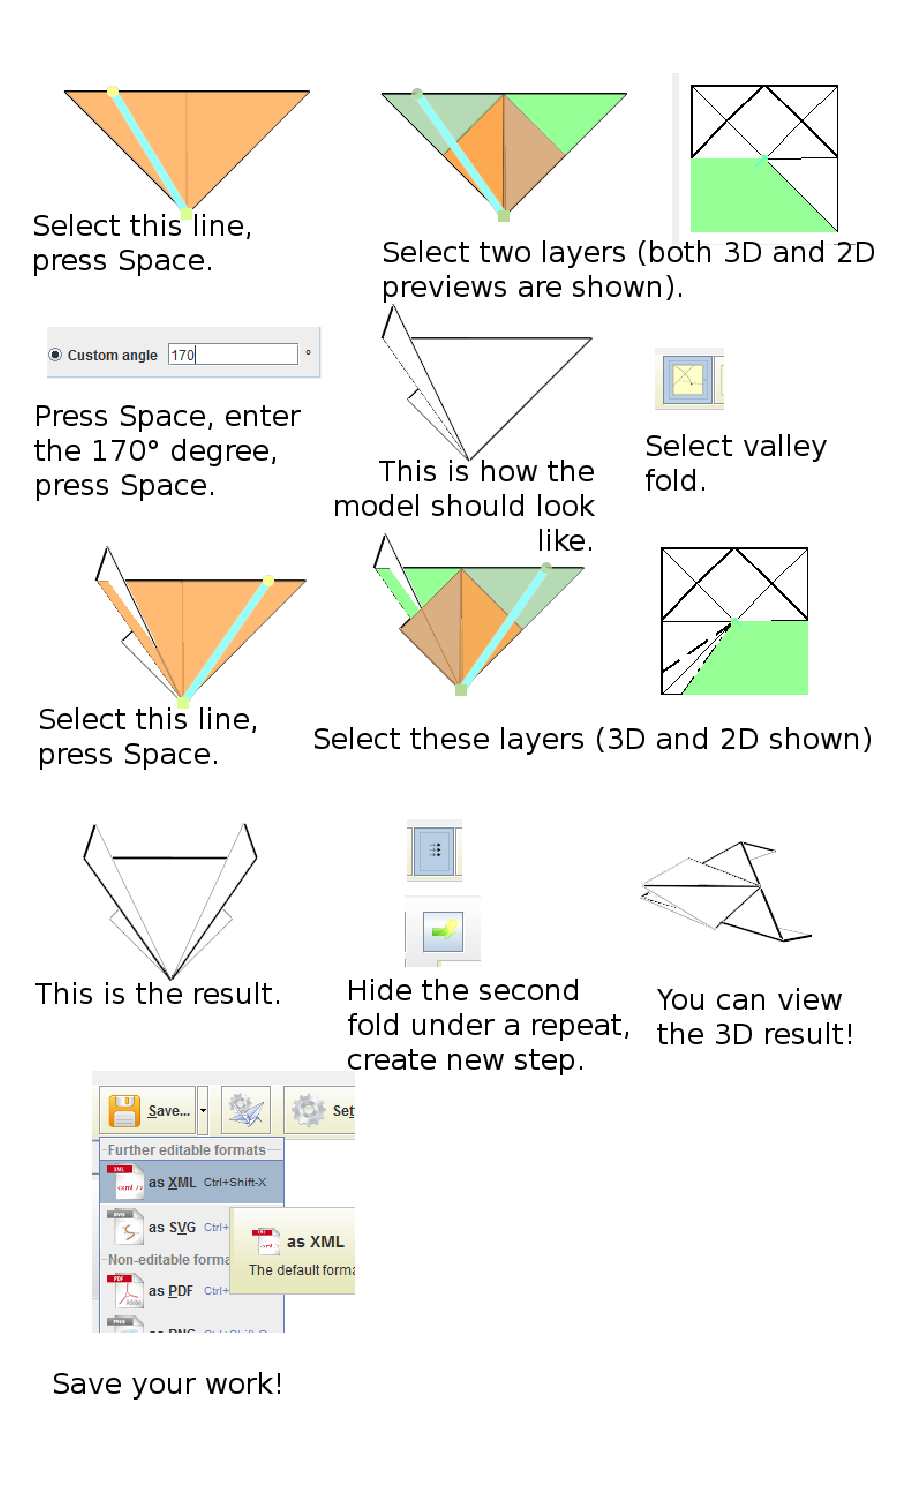
\includegraphics[width=140mm]{images/frog-tutorial3}
	\label{fig:tutorial3}
	\caption{Frog base tutorial, part 3}
\end{figure}
